\chapter{Evaluation}\label{ch:evaluation}

\section{Prequisites}

\section{Browser compatbility}
\begin{table}[!htb]
\begin{center}

	\begin{tabular}{|l|l|l|l|l|}
		\hline
		Chrome & Firefox & Edge & Safari & Internet Explorer	  \\ \hline
		75 	   & 68 	  & 76	 & 12.1	  & Not supported    				\\ \hline
	\end{tabular}
	
	\begin{tabular}{|l|l|l|l|l|}
		\hline
		IOS Safari & Samsung Internet & Android Browser	& Chrome (Android) \\ \hline
		12.3	   & 9.2				  & 67				& 75  \\ \hline
	\end{tabular}

	\caption{Unterstützte Browser Versionen}
\end{center}

Um die unterstützten Browser zu verifizieren wurden die vom \pTp \cdn verwendeten Browser Funktionalitäten bei caniuse.com\footnote{https://caniuse.com/} eingegeben. Darüber hinaus wurden Chrome, Firefox, Edge, Safari und der Internet Explorer manuell getestet, um sicherzustellen das das \pTp \cdn das Nutzererlebnis nicht negativ beeinflusst. Der Internet Explorer unterstütz auch in der aktuellen Version keine Service Worker\footnote{https://caniuse.com/#search=service\%20worker}. Auch wenn der Edge Browser Webrtc seit Version 17 unterstützt, ist es leider erst ab version 76 möglich Datachannels zu verwenden. Da der Datenverkehr des \pTp \cdns über Datachannel gehandhabt wird, ist eine Verwendung erst ab der nächsten Version die auf Chrome aufbauen wird, möglich.
\end{table}

\subsection{Browser Usage in coropate networks}

\begin{itemize}
	\item Statistic über typische nutzung
	\item Statistic über Nutzung bei dem test
	\item Diskussion Edge on Chromium
	\item evtl aussage von deutscher bank mit aufnehmen
	\item  --- major update hinauszögern, in 1-2 Jahren
	\item 
\end{itemize}


\subsection{Browser usage in eduational networks}
\begin{itemize}
	\item evtl einfach normale verteilung
	\item schauen ob es quellen gibt
\end{itemize}
\section{Webrtc Routing}
\begin{itemize}
	\item mit und ohne STUN
	\item lokales routing
	\item externes Routing
	\item implikationen für Konfiguration
\end{itemize}
\section{Bandwidth}



\subsection{Latency}

\subsubsection{Webrtc Verbindungsaufbau}

\begin{itemize}
	\item Page load bis cdn is ready
	\item verschiedene Anzahl an Peers im Netzwerk 
\end{itemize}

\section{Simulierter Workload}
\subsection{Chunking}
\begin{itemize}
	\item messen des aufwandes für chunking und wieder zusammensetzen
	\item woher kommt der zusätzliche Aufwand bei größen dateien??
	\item limit ist der durchsatz nicht das chunking
\end{itemize}

\subsection{Durchsatz - Ladezeiten von verschiedenen Dateigrößen}
Um die Ladezeiten verschiedener Dateigrößen zu evaluieren wurde auf einem Mac book pro Ende 2013 mit 2.3 GHz und 16GB Arbeitsspeicher getestet. 
Getestet wurde mit zwei Teilnehmern. Einer lud die Ressource vor und der zweite lud sie über das \pTp \cdn. Die Timeouts des \pTp \cdns wurden für diesen Test deaktiviert. Um Netzlaufzeiten auszuklammern befand sich der Anwendungsserver ebenso wie die zu ladene Ressource auf dem selben Rechner wie die Clients. 

\begin{figure}[!h]
	\centering
	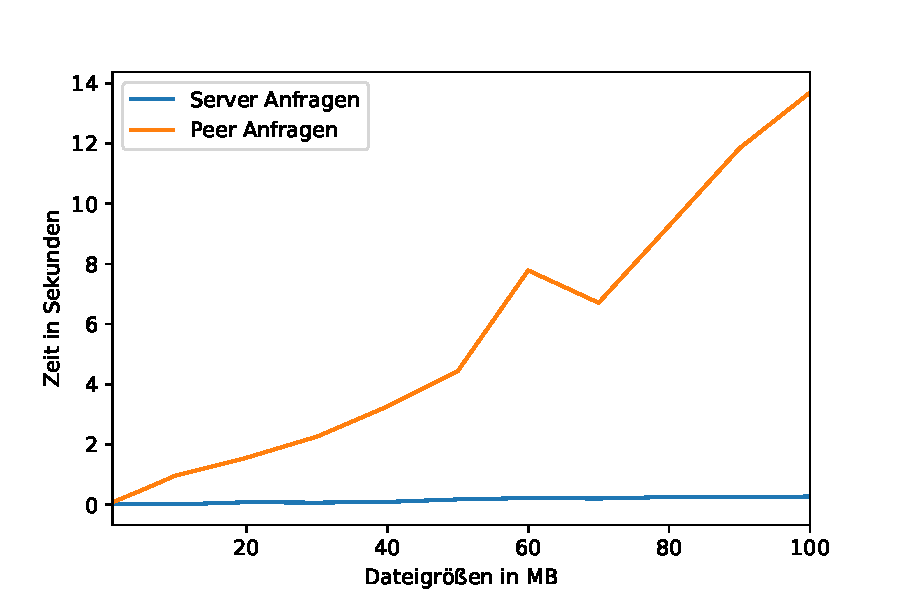
\includegraphics[width=0.8\textwidth]{figures/Timing_file_size}
	\caption[A Figure Short-Title]{}
	\label{fig:timing_file_size}
\end{figure}

\begin{figure}[!h]
	\centering
	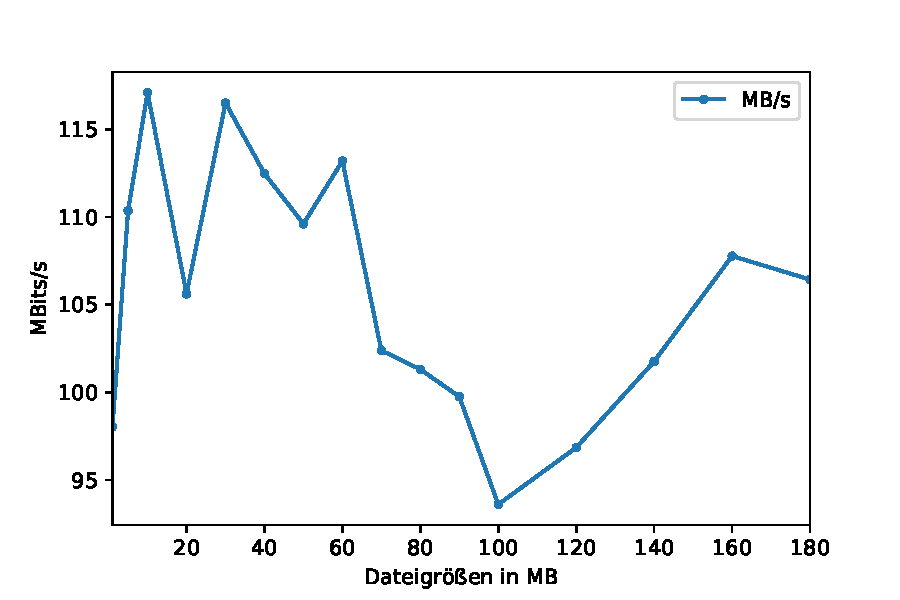
\includegraphics[width=0.8\textwidth]{figures/durchsatz_file_size}
	\caption[A Figure Short-Title]{Durchsatz}
	\label{fig:durchsatz_file_size}
\end{figure}


\begin{itemize}
	\item Mac book pro Ende 2013
	\item 2.3 ghz i7
	\item 16gb ram
	\item 1, 5, 10, 20, 30, 40, 50, 60, 70, 80, 90 , 100 mb
	\item durchsatz berechnen
	\item Limitierung durch websockets
	\item lokal auf einem Rechner um Netzlaufzeiten auszuklammern
	\item 1 Peer lädt vor
	\item der andere lädt von peer
	\item benchmarkt das nur das lokale netzwerk?? --> routing
	\item sicherstellen das datenverkehr nicht über internet geroutet werden...
\end{itemize}

\subsection{Live Streaming}
Um einen Live Stream mit höherer Teilnehmerzahl zu testen wurde ein Script geschrieben, das mit Hilfe von puppeteer\footnote{TODO: puppeteer} mehrere Chrome browser um headless Mode startet und die Event Seite besucht. Dabei musste eine Chrome installation gewählt werden, da Chromium nicht über die notwendigen Codecs verfügt um HLS Video wieder zu geben. 
Das Script wurde auf Amazon AWS t2.xlarge Instanzen installiert. Jede dieser Instanzen verfügt über 8 vcpus und 32 GB Arbeitsspeicher. Auf jeder Instanz wurden 25 Browser Sessions geöffnet.  Das \cdn wurde so konfiguriert das es ausschließlich .ts Dateien, also die Video Segmente bearbeitet. Bei 25 Teilnehmern lag die CPU Last bei den Testservern bei deaktiviertem \pTp \cdn bei 50-60\%. 
Die Teilnehmer luden die Event Seite während das Event noch nicht Live geschaltet war. Wenn alle Teilnehmer die Seite geladen hatten wurde das Event live geschaltet und die Teilnehmer auf die Live stream Seite weiter geleitet. Die Weiterleitung geschieht verzögert in einem Zeitraum von 18-60 Sekunden mit einer Dreicks-verteilung um die Last auf Seiten der Slidesync Servern zu verringern Der Stream wurde für zehn Minuten live geschaltet und anschließend beendet.

\begin{figure}[!h]
	\centering
	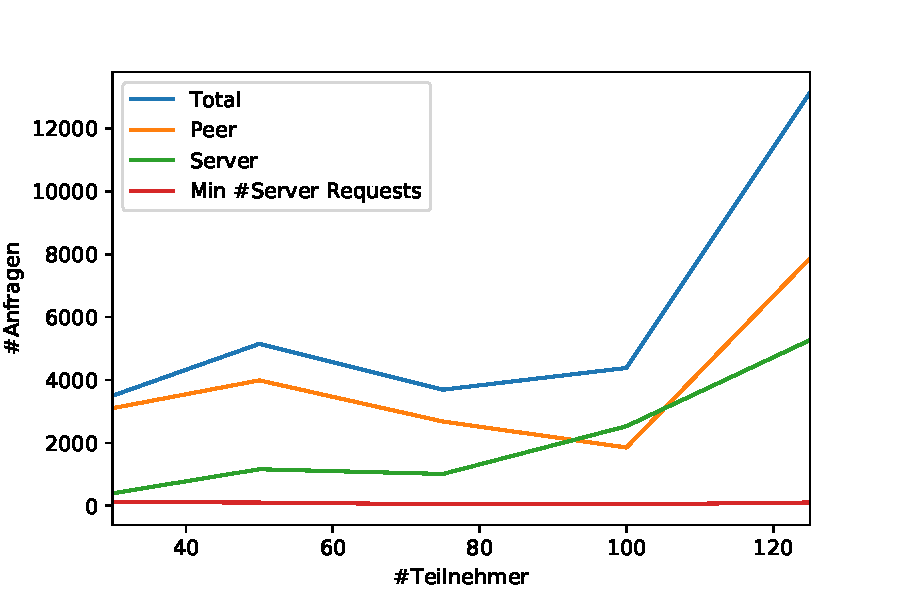
\includegraphics[width=0.8\textwidth]{figures/single_mesh_line}
	\caption[A Figure Short-Title]{Vergleich der Bearbeitung nach Art in einem Mesh}
	\label{fig:single_mesh_line}
\end{figure}
\todo{Datenpunkte mehr ersichtlich machen}

Abbildung \ref{fig:single_mesh_line} zeigt die wie sich das \pTp \cdn bei steigender Teilnehmerzahl mit einem Mesh verhält. Bis 50 Teilnehmern hat das \cdn ein lineares Verhalten hinsichtlich bearbeiteter Anfragen. Ab 75 Teilnehmern ist zu sehen das die Gesamtanzahl der verarbeiten Anfragen einbricht. Die CPU Last der Test Server stieg auf 100\% und die Clients waren dadurch nicht mehr in der Lage an dem \cdn Teilzunehmen und Anfragen zu bearbeiten. Der Kommunikationsaufwand die Peers in dem Mesh über Veränderungen des Caches zu Benachrichtigen wurde zu groß. Zwar wurden bei 125 Teilnehmern wieder mehr Anfragen vom \cdn verarbeitet, jedoch stieg der Anteil der Anfragen die über den Server liefen weiter an. Die höhere Anzahl an Anfragen die vom \cdn bearbeitet wurden ist vor allem darauf zurück zu führen, dass die Verbindungen zwischen den Peer durch die hohe Last teilweise unterbrochen wurde, wodurch sich die Last bei den Teilnehmern verringerte.   

\begin{figure}[!h]
	\centering
	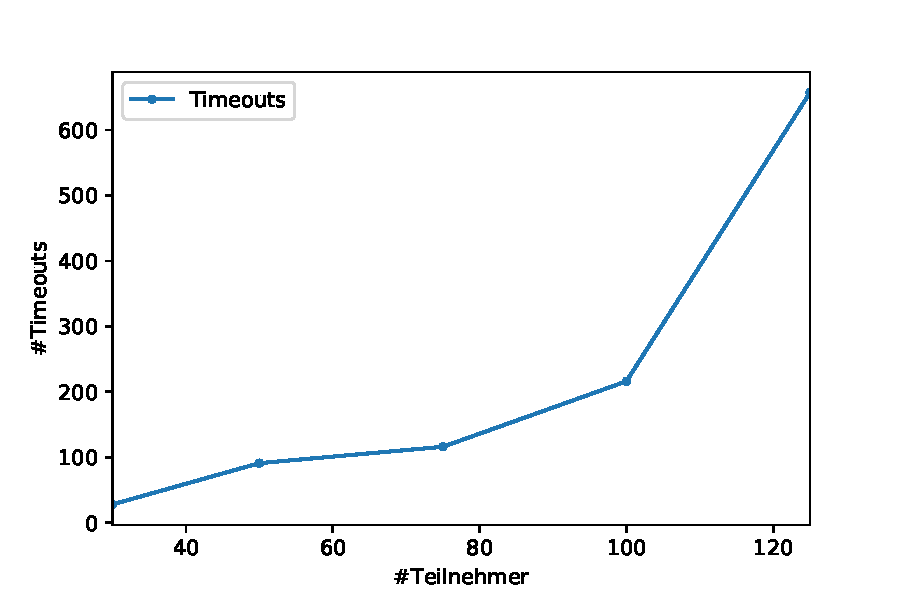
\includegraphics[width=0.8\textwidth]{figures/timeouts_single}
	\caption[A Figure Short-Title]{Timeouts bei einem Mesh}
	\label{fig:timeouts_single}
\end{figure}

Betrachtet man die Anzahl an Timeouts, so bestätigen sich die vorherigen Beobachtungen. Ab 75 Teilnehmern steigt die Anzahl an Timeouts stark an. Die CPU Last auf Seiten der Teilnehmern wurde zu groß um alle Anfragen in der geforderten Zeit zu beantworten. Neben der zu hohen Last ist kann es zu Timouts kommen falls zu viele Teilnehmer gleichzeitig eine Anfrage an den Selben Teilnehmer stellen. Der betroffene Teilnehmer ist in diesem Fall nicht in der Lage alle Anfragen schnell genug zu bearbeiten. Der Timeout wurde mit drei Sekunden so gewählt das es trotz Timeouts nicht zu einer Unterbrechung des Streams kommt. Der Video Player von Slidesync lädt drei HLS vor die je sechs Sekunden Video beinhalten insgesamt werden also 18 Sekunden vor geladen. Zu einer Unterbrechung der Wiedergabe kann es also erst kommen wenn eine Anfrage länger als 6 Sekunden benötigt. Da die längste verarbeitete Anfrage XXX Sekunden benötigte kam es zu keiner Unterbrechung der Wiedergabe aufgrund von Timeouts.

\begin{figure}[!h]
	\centering
	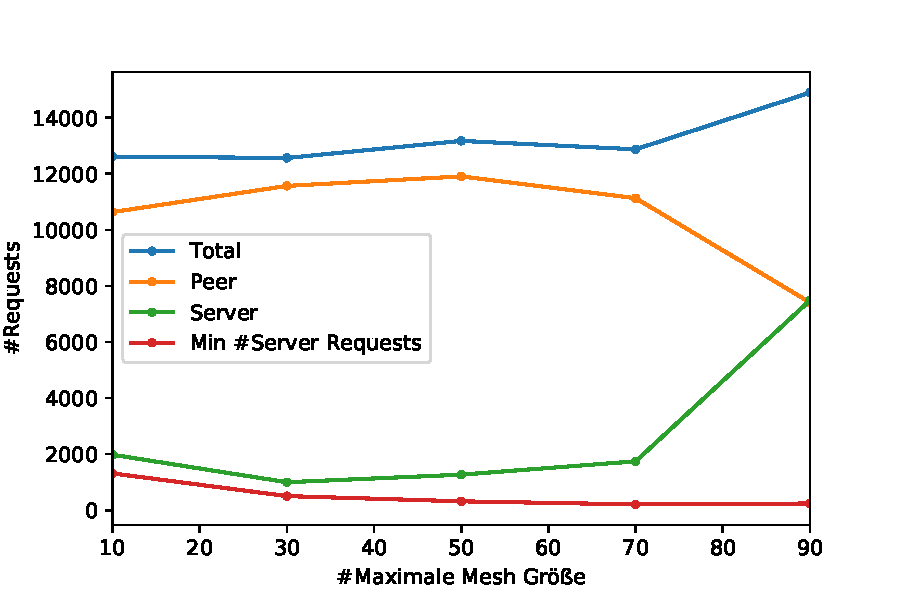
\includegraphics[width=0.8\textwidth]{figures/mesh_comparison}
	\caption[A Figure Short-Title]{Vergleich verschiedener Mesh Größen}
	\label{fig:mesh_comparison}
\end{figure}

\begin{figure}[!h]
	\centering
	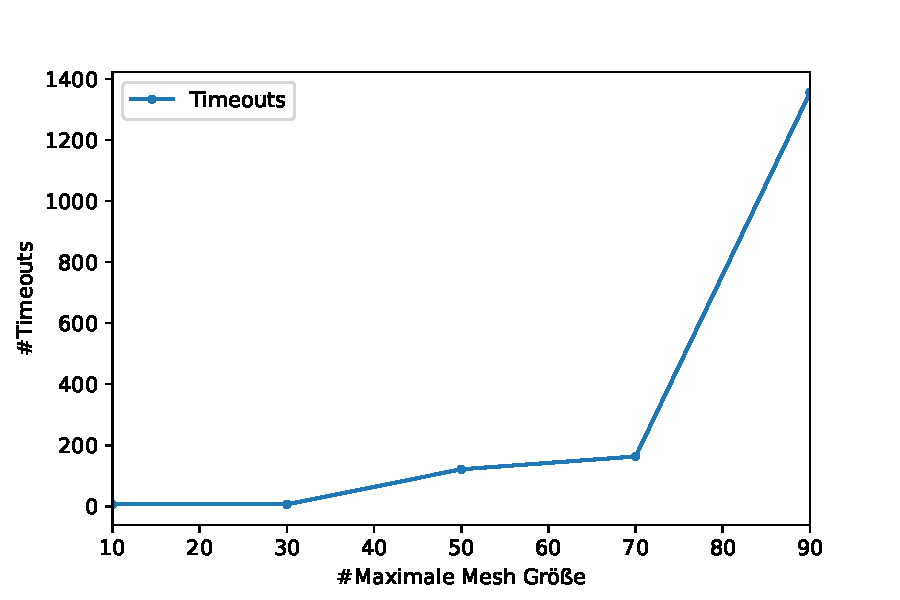
\includegraphics[width=0.8\textwidth]{figures/timeouts_meshed}
	\caption[A Figure Short-Title]{#Timeouts bei verschiedenen Mesh Größen (125 Teilnehmer)}
	\label{fig:timeouts_meshed}
\end{figure}

Abbildung \ref{fig:mesh_comparison} zeigt die Verarbeitungsart der Anfragen bei steigender Mesh Größe. Alle Tests wurden mit einer Teilnehmerzahl von 125 durchgeführt. Bei einer Mesh Größe von zehn ist die mindestanzahl an Anfragen die von dem Server beantwortet werden müssen mit 10\% relativ groß. Auch wenn nur selten Timeouts durch zu viele Anfragen bei dem selben Teilnehmer vorkommen konnten nur 84\% der Anfragen über das \pTp \cdn beantwortet werden. Die Beste Abdeckung hatte das \cdn bei einer Mesh Größe von 30 Teilnehmern mit 92\%. Bei einer Mesh Größe sind müssen mindestens 4\% der Anfrage über den Server beantwortet werden, damit jedes HLS Segment in jedem Peer Mesh vorhanden ist. Wird eine größere Mesh Größe als 30 gewählt so steigt auch die Anzahl der Timeouts ebenso wie die CPU Auslastung bei den Teilnehmern. So konnte bei einer Mesh Größe von 90 lediglich die Hälfte aller Anfragen durch das \pTp \cdn beantwortet werden.


\begin{figure}[!h]
	\centering
	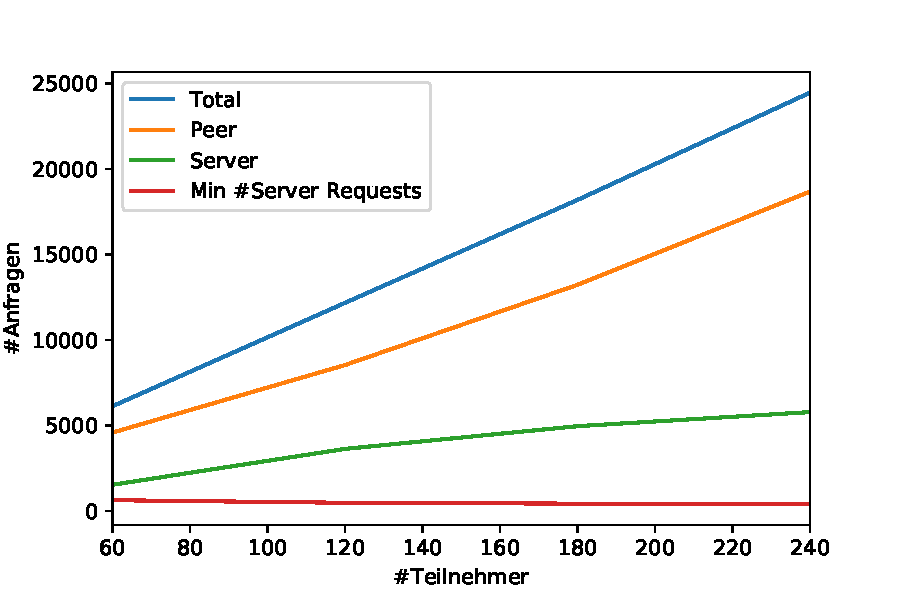
\includegraphics[width=0.8\textwidth]{figures/meshed_30_line}
	\caption[A Figure Short-Title]{Mesh Größe von 30 bei steigender Teilnehmer Zahl}
	\label{fig:meshed_30_line}
\end{figure}

Um zu testen wie sich das \cdn bei größeren Teilnehmerzahlen verhält wurden Tests mit einer Mesh Größe von 30 durchgeführt. Abbildung \ref{fig:meshed_30_line} zeigt einen Vergleich der Verarbeitungsarten. Die Anzahl an Peer Anfragen Verhält sich linear mit steigender Teilnehmerzahl. Die Abdeckung durch das \cdn schwankt zwischen 70-76\%.


\begin{figure}[!h]
	\centering
	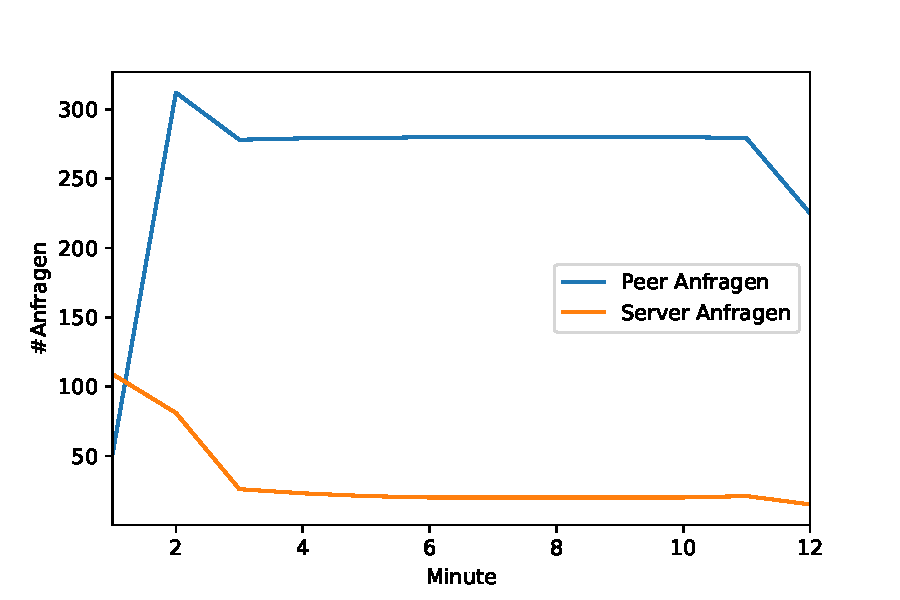
\includegraphics[width=0.8\textwidth]{figures/peer_vs_server_over_time}
	\caption[A Figure Short-Title]{Anfrageart über die Zeit bei 30 Teilnehmern}
	\label{fig:peer_vs_server_over_time}
\end{figure}

Abbildung \ref{fig:peer_vs_server_over_time} zeigt eine zeitliche Darstellung von beginn des Streams bis zum Ende des Streams für 30 Teilnehmer in einem Mesh. Es ist gut zu sehen, dass zu Beginn des Tests mehr Anfragen über die Server beantwortet werden müssen. Auch die Gesamtanzahl der Anfragen ist zu beginn des Tests höher als im späteren Verlauf. Nachdem die Seite geladen ist laden alle Teilnehmer drei HLS Segemente vor. Diese HLS Segmente werden gleichzeitig geladen, wodurch sich die Wahrscheinlichkeit erhöht das mehere Teilnehmer annähernd gleichzeitig die selbe Ressource anfragen und kein anderer Teilnehmer sie bereits geladen hat. 


\todo{Rahmenbedingungen müssen klar sein}


\begin{itemize}
	\item Verhältnisse berechnen
	\item evtl ramp up anschauen
	\item  
\end{itemize}

\begin{itemize}
	\item 92872 pro segment (ca 92 kb) 
	\item ca 9,2 mb pro client pro event
	\item bandbreiten diagram? 
	\item Wenn client von server lädt teilt er das direkt mit
\end{itemize}

\subsection{Schul-Cloud}

\begin{itemize}
	\item Testsetup
	\item 30 Schüler
	\item 3 Clicks
	\item Dashboard
	\item kurs liste
	\item kurs
	\item Thema
	\item hauptsächlich css etc
	\item 1 Server macht anfragen
	\item verschieden zufällig gewählte startzeiten in verschiedenen Zeiträumen
	\item wo turbolinks erwähnen?
\end{itemize}
\begin{figure}[!h]
	\centering
	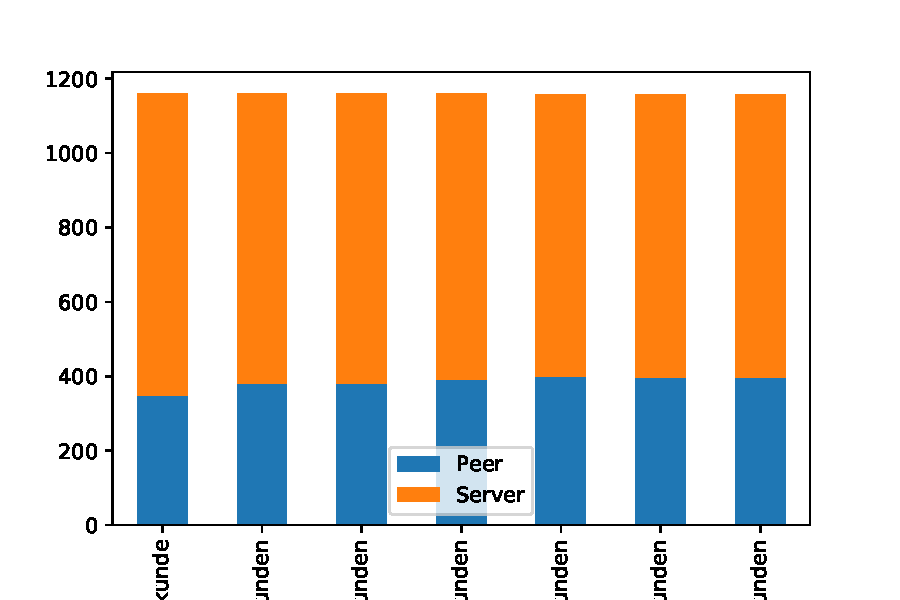
\includegraphics[width=0.8\textwidth]{figures/sc_stacked_interval}
	\caption[A Figure Short-Title]{Vergleich der Anfragen nach Anfrageart}
	\label{fig:15_clients_network}
\end{figure}

\begin{itemize}
	\item Kein Großer unterschied zwischen den Zeiträumen
\end{itemize}

\begin{figure}[!h]
	\centering
	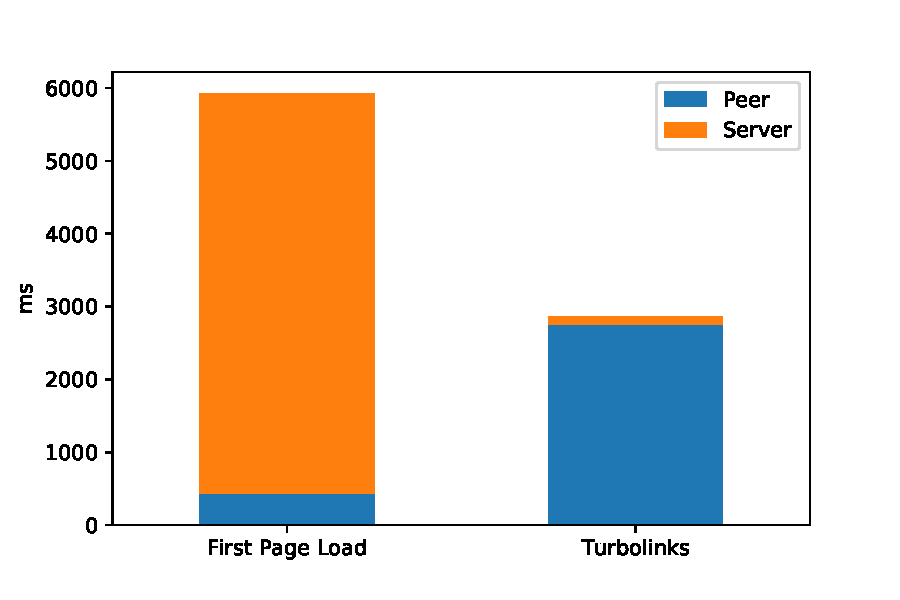
\includegraphics[width=0.8\textwidth]{figures/sc_first_vs_later}
	\caption[A Figure Short-Title]{Vergleich der Anfragen nach Anfrageart}
	\label{fig:15_clients_network}
\end{figure}
\todo{Beschriftungen}

\begin{itemize}
	\item First load vs navigationen
	\item First load schlechte abdeckung -> erst möglich wenn cdn initialisiert ist
	\item navigationen sehr hohe abdeckung
	\item swa/turbolinks notwendig
\end{itemize}


\begin{itemize}
	\item weiteres szenario 
	\item 1 User hat geladen(Lehrer)
	\item rest kommt
	\item inhalt mit pdf

\end{itemize}

\section{Livestreaming in Unternehmensnetzwerken}

Um die Funktionalität des \cdns im Falle eines Livestreams zu testen wurde ein Livestream mit der Infrastruktur von Slidesync aufgesetzt. Slidesync verwendet bei der Verteilung des Videos das Datenformat HLS. Das \cdn wurde so konfiguriert das ausschließlich die HLS Segmente über das \cdn behandelt werden. Sämtliche im folgenden betrachteten Anfragen sind demnach HLS Segmente. 
\begin{figure}[!h]
	\centering
	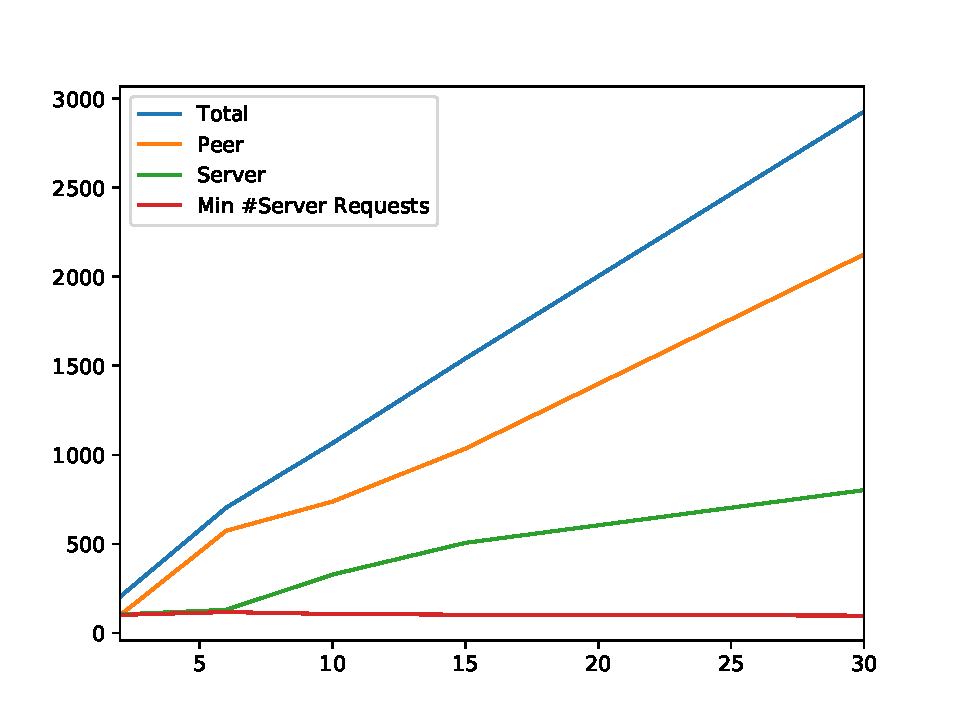
\includegraphics[width=0.8\textwidth]{figures/clients_line_chart}
	\caption[A Figure Short-Title]{Vergleich der Anfragen nach Anfrageart}
	\label{fig:live_stream_line_chart}
\end{figure}
Der Test wurde in einem Unternehmensnetzwerk durchgeführt um die Funktionalität in einem solchen Netzwerk zu gewährleisten. In diesem Netzwerk wurden insgesamt 30 Rechner aufgestellt. Da es vor allem um den Durchsatz des \cdns ging wurde auf allen Clients ein aktueller Chrome Browser verwendet. Auf den Clients wurde zuerst die Event Seite geladen und erst im Anschluss der Livestream gestartet. Getestet wurden sechs, zehn, 15, 20 und 30 Clients, die sich alle im selben lokalen Netzwerk befanden. Der Streaming- und der Anwendungsserver befand sich außerhalb des Netzwerkes und waren nur über die Internetverbindung zu erreichen. Bei jedem Test wurde der Stream zehn Minuten laufen gelassen und alle Clients befanden sich in dem selben Peer Mesh.

\begin{figure}[!h]
	\centering
	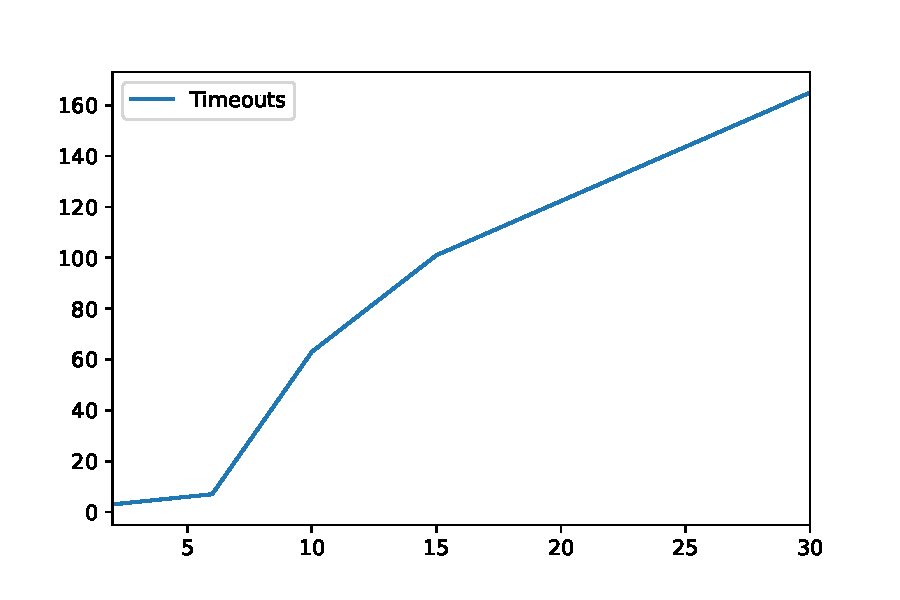
\includegraphics[width=0.8\textwidth]{figures/timeouts}
	\caption[A Figure Short-Title]{Anzahl der Timeouts des \cdns}
	\label{fig:timeouts}
\end{figure}


Abbildung \ref{fig:live_stream_line_chart} zeigt die Abhandlungsart der Anfragen. Dabei ist zu beachten das ca 100 Requests notwendig waren damit sämtliche HLS Segmente im \pTp Netzwerk verfügbar sind. Bei steigender Anzahl von Teilnehmern ist zu beobachten das eine größere Anzahl an Anfragen über den Server geladen werden müssen. Ein möglicher Grund hierfür ist Die Zeitliche Verteilung der Anfragen. Befinden sich mehr Peers im Netzwerk so wird es wahrscheinlicher das zwei Teilnehmer sich beide an der selben Stelle im Video befinden, die HLS Segmente laden müssen, jedoch noch kein Teilnehmer das Segment heruntergeladen hat. Auch wird es wahrscheinlicher das eine größere Anzahl an Teilnehmern ein Segment über den selben Teilnehmer laden wollen. Fragen zu viele Teilnehmer eine Ressource bei selben Teilnehmer an, so kann er nicht mehr alle Anfragen bearbeiten. Die Anfrage über das \pTp \cdn wird abgebrochen und über den Server geladen. Abbildung \ref{fig:timeouts} zeigt die Anzahl der Timeouts bei steigender Teilnehmerzahl. Dabei ist zu beachten das der Timeout so gewählt wurde das das Video weiterhin flüssig lief.

\begin{figure}[!h]
	\centering
	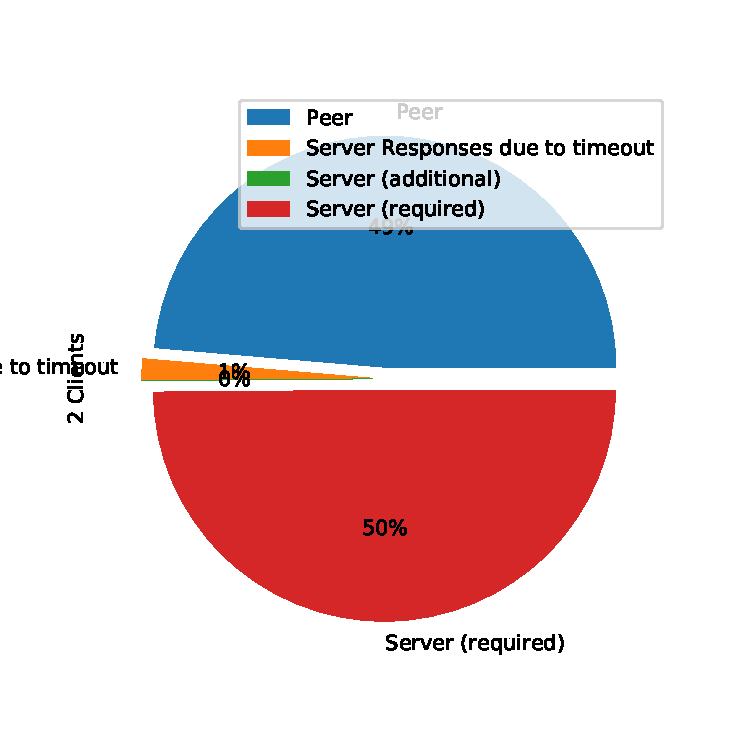
\includegraphics[width=0.45\textwidth]{figures/pie_2_clients}
	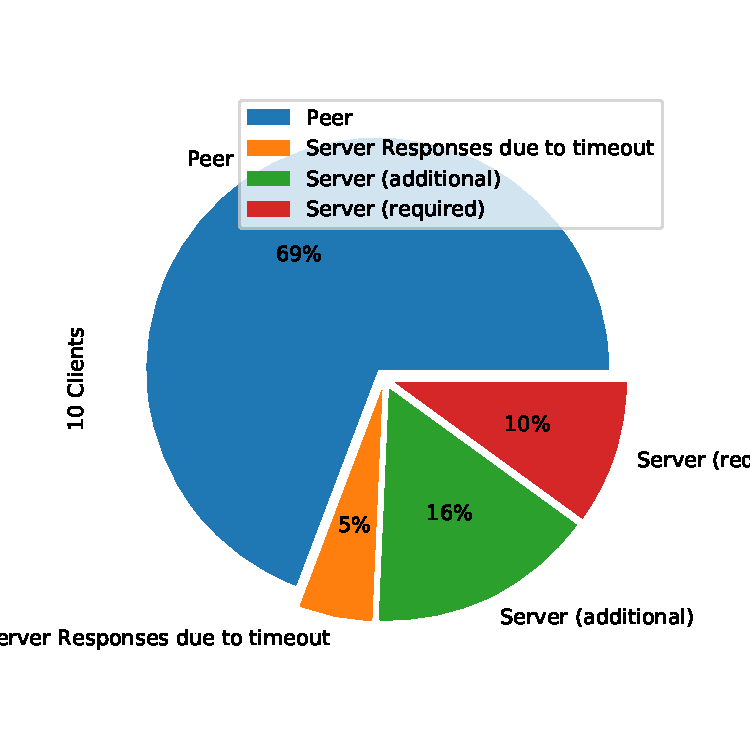
\includegraphics[width=0.45\textwidth]{figures/pie_10_clients}
	\caption[A Figure Short-Title]{Verteilung der Anfragen bei zwei und 10 Clients}
	\label{fig:corporate_pie_2}
\end{figure}
\begin{figure}[!h]
	\centering
	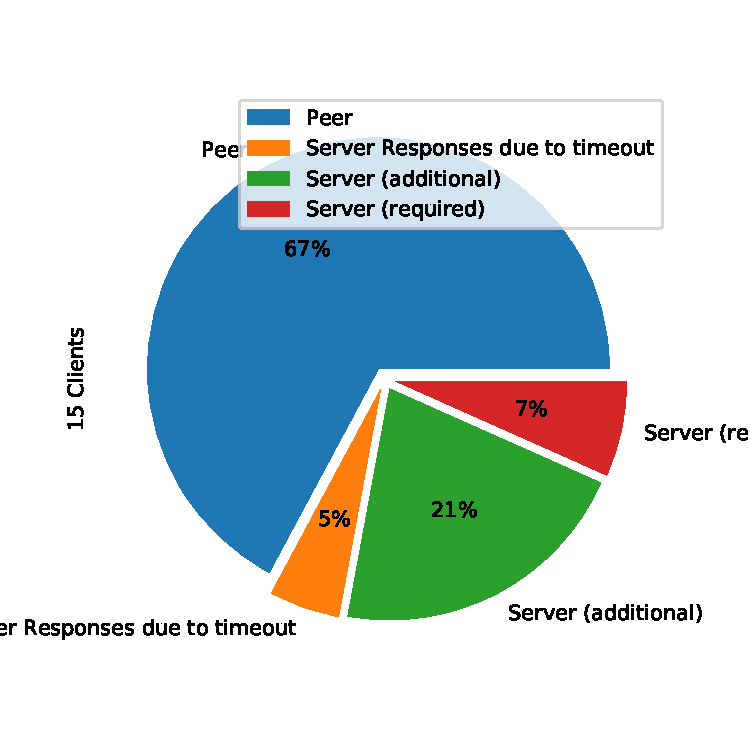
\includegraphics[width=0.45\textwidth]{figures/pie_15_clients}
	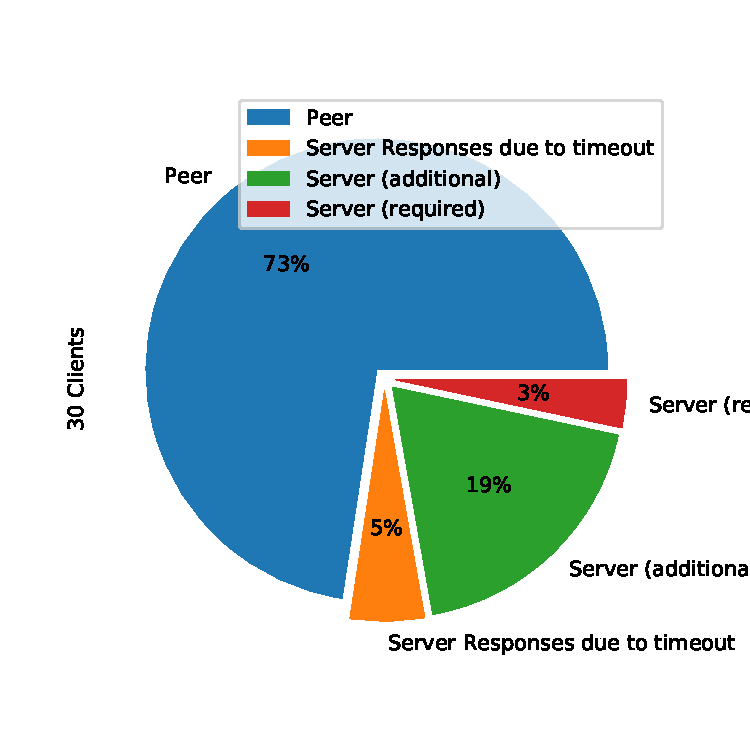
\includegraphics[width=0.45\textwidth]{figures/pie_30_clients}
	\caption[A Figure Short-Title]{Verteilung der Anfragen bei zwei und 10 Clients}
	\label{fig:corporate_pie_3}
\end{figure}

Betrachtet man die zusätzlich Notwendigen Server Anfragen so lässt sich beobachten das der Prozentsatz in diesem Test annähernd konstant ist.  

%\begin{figure}[!h]
%	\centering
%	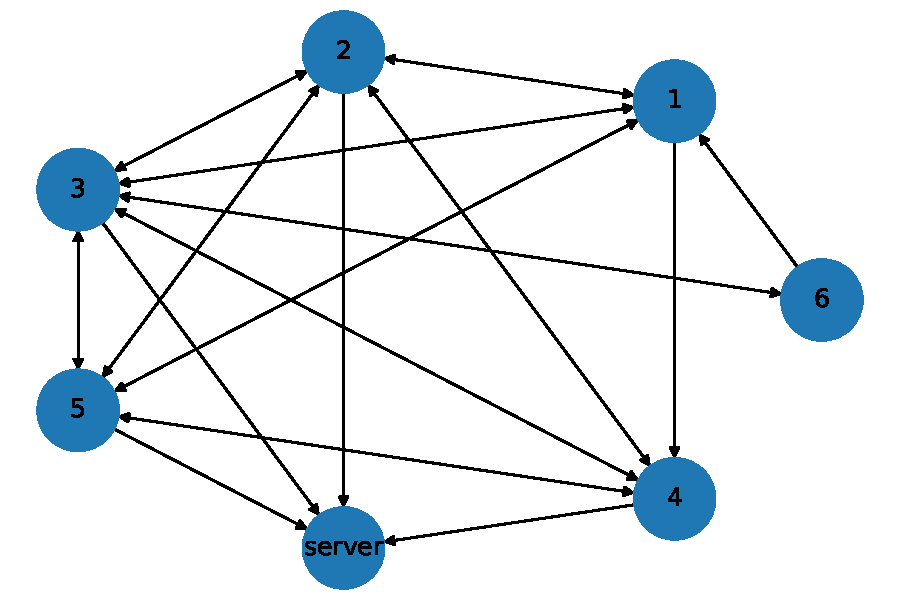
\includegraphics[width=0.8\textwidth]{figures/6_clients_network}
%	\caption[A Figure Short-Title]{Vergleich der Anfragen nach Anfrageart}
%	\label{fig:6_clients_network}
%\end{figure}

\begin{figure}[!h]
	\centering
	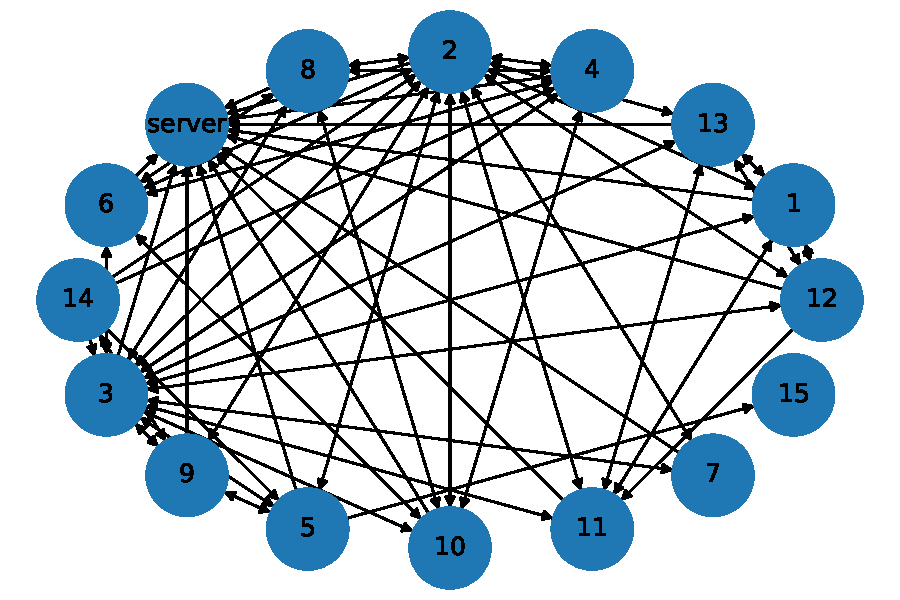
\includegraphics[width=0.8\textwidth]{figures/15_clients_network}
	\caption[A Figure Short-Title]{Vergleich der Anfragen nach Anfrageart}
	\label{fig:15_clients_network}
\end{figure}

Abbildung \ref{fig:15_clients_network} zeigt welche Teilnehmer untereinander Daten ausgetauscht haben. Auffällig ist das einige Teilnehmer besonders vielen Teilnehmern Daten gesendet haben. Dies war besonders dann der Fall wenn sie die einzigen im Netzwerk waren die das Segment bereits geladen hatten. Die meisten Kanten sind jedoch bidirektional, sprich zwar haben einige Teilnehmer besonders viele Anfragen beantwortet, jedoch haben sie sich nicht als zentrale Punkte des Netzwerkes etabliert sondern ebenfalls ihre Daten von anderen Teilnehmern geladen. \todo{gewichtung??} 

\begin{table}[!htb]
\begin{center}

	\begin{tabular}{|r|l|l|l|l|l|l|}
		\hline
		Request Art	 & #Anfragen 	& Durchschnitt 	& Standardbweichung	& Min		& Max	 \\ \hline
		Peer 		& 4571 				& 201.60	 ms	  	& 190.14	 ms				& 27.02 ms	& 2832.27 ms \\ \hline
		Server 		& 1870		 		& 63.61 ms		& 62.99	ms				& 9.41 ms	& 649 ms	\\
		\hline
	\end{tabular}
	\caption{Browser Storage Quotas }
\end{center}

\end{table}

Bei der Betrachtung der Ladezeiten wurden alle erfassten Anfragen berücksichtigt. Allerdings wurden die Daten um die Server Anfragen bereinigt bei denen zuvor das \pTp \cdn einen timeout verursacht hat. Insgesamt wurden 4571 Peer Anfragen und 1870 Server Anfragen betrachtet. 
Anfragen die vom \pTp \cdn beantwortet wurden brauchten im Durchschnitt 201,60ms. Server Anfragen waren im Vergleich mit 63,31ms im Durchschnitt deutlich schneller. Die ist auf den geringeren Durchsatz der \webrtc Datachannels zurückzuführen. (Siehe Dateigrößen \todo{ref}) Damit war das \pTp \cdn zwar deutlich langsamer, jedoch schnell genug um eine flüssige Wiedergabe zu gewährleisten. Da eine Anfrage die länger als 3000ms brauchte bei dem \pTp \cdn zu einem timeout geführt hat betrug die höchste erfasste Ladezeit 2832,27 ms.    
%\todo{einige clients haben keine daten an den server gesendet. Rausrechnen!}
%\begin{itemize}
%	\item ladezeiten
%	\item Alle Anfragen berücksichtigt
%	\item 4571.0 peerRequest
%	\item serverResponse   1870.0
%	\item Serveranfragen bereinigt um die Timeouts
%\end{itemize}
\begin{itemize}
	\item andere auflösungen
	\item s vs p
	\item server downloadtime berücksichtigen
	\item besonders vergleich für hohe auflösungen
	\item vergleich verschiedener Auflösungen
\end{itemize}
%passt hier nicht wirklich hin